\begin{frame}{Adgang til Våben: Jagttegn og Tilladelser}

\vspace{1em}

\begin{columns}[c] % c = center vertically

\column{0.05\textwidth} % Venstre margin

\column{0.7\textwidth} % Midten: Bullets

\small

\raggedright

\begin{itemize}

\itemsep0.6em % Justér afstand mellem bullets

\item Et jagttegn udstedes kun med \textbf{samtykke fra Politiet} (vurdering af vandel/egnethed, jf. § 6).

\item Du skal være fyldt \textbf{18 år} for selv at kunne \structure{erhverve} og \structure{besidde} skydevåben.

\item Våben må kun håndteres af personer, der kan fremvise \textbf{gyldigt jagttegn} eller \structure{våbentilladelse} (§ 20).

\item Du må bruge haglgevær under \structure{jagtprøven} og til instruktion, da kursuslærere må overlade våben til dig (§ 21).

\item \textbf{Ungjægerordningen}: Er du under 18 år, skal du jage \textbf{i følge med} en myndig jæger (over 18 år).

\end{itemize}

\column{0.25\textwidth} % Højre: Ikon

\centering

\vspace{0pt}

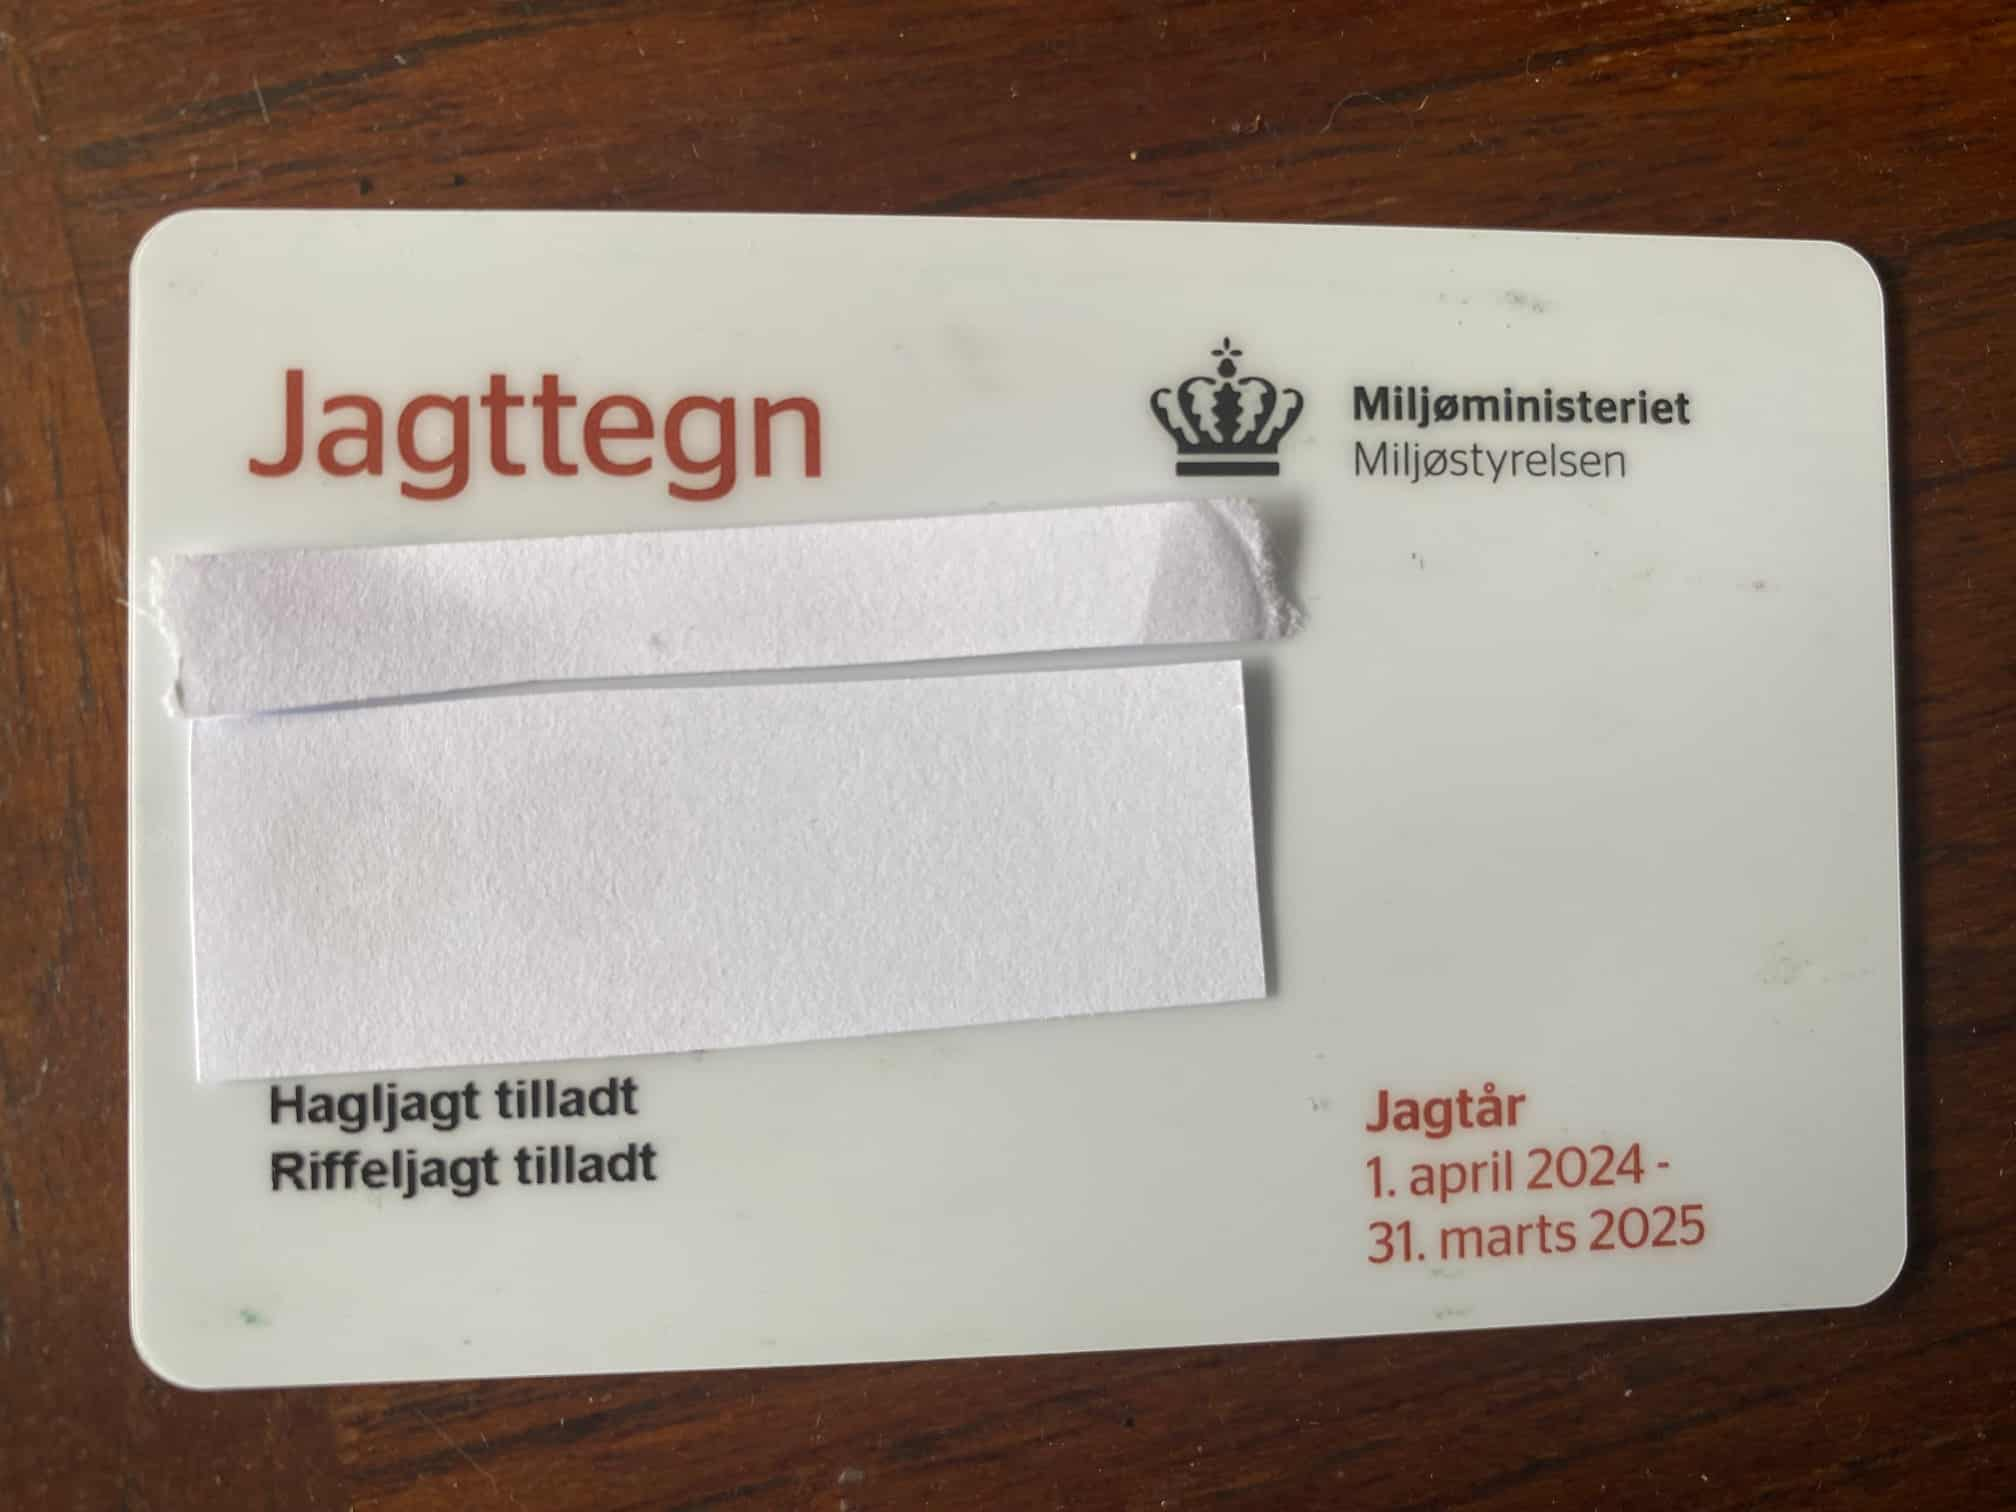
\includegraphics[width=0.9\linewidth]{Billeder/Redskaber/jagttegn_billede.jpg} % Antager et ikon, der passer til 'Tilladelse' (evt. et jagttegn)

\end{columns}

\end{frame}